\documentclass[twoside]{report}
\usepackage{graphics}
\usepackage[utf8]{inputenc}
\setlength{\oddsidemargin}{0.25 in}
\setlength{\evensidemargin}{-0.25 in}
\setlength{\topmargin}{-0.2 in}
\setlength{\textwidth}{6.5 in}
\setlength{\textheight}{8.5 in}
\setlength{\headsep}{0.0 in}
\setlength{\parindent}{0 in}
\setlength{\parskip}{0.1 in}

%
% The following commands set up the lecnum (lecture number)
% counter and make various numbering schemes work relative
% to the lecture number.
%
\newcounter{lecnum}
\newcounter{qnum}
\renewcommand{\thepage}{\thelecnum-\arabic{page}}
\renewcommand{\thesection}{\thelecnum.\arabic{qnum}}
\renewcommand{\theequation}{\thelecnum.\arabic{equation}}
\renewcommand{\thefigure}{\thelecnum.\arabic{figure}}
\renewcommand{\thetable}{\thelecnum.\arabic{table}}

%
% The following macro is used to generate the header.
%
\newcommand{\lecture}[4]{
   \pagestyle{myheadings}
   \thispagestyle{plain}
   \newpage
   \setcounter{lecnum}{#1}
   \setcounter{page}{1}
   \setcounter{qnum}{8}
   \noindent
   \begin{center}
   \framebox{
      \vbox{\vspace{2mm}
    \hbox to 6.28in { {\bf EE 382V: Social Computing
                        \hfill Fall 2018} }
       \vspace{4mm}
       \hbox to 6.28in { {\Large \hfill #2  \hfill} }
       \vspace{2mm}
       \hbox to 6.28in { { \hfill Scribe: #4} }
      \vspace{2mm}}
   }
   \end{center}
   \markboth{#2}{#2}
   %{\bf Disclaimer}: {\it These notes have not been subjected to the
   %usual scrutiny reserved for formal publications.  They may be distributed
   %outside this class only with the permission of the Instructor.}
   \vspace*{4mm}
}

%
% Convention for citations is authors' initials followed by the year.
% For example, to cite a paper by Leighton and Maggs you would type
% \cite{LM89}, and to cite a paper by Strassen you would type \cite{S69}.
% (To avoid bibliography problems, for now we redefine the \cite command.)
% Also commands that create a suitable format for the reference list.

\renewcommand{\cite}[1]{[#1]}
\def\beginrefs{\begin{list}%
        {[\arabic{equation}]}{\usecounter{equation}
         \setlength{\leftmargin}{2.0truecm}\setlength{\labelsep}{0.4truecm}%
         \setlength{\labelwidth}{1.6truecm}}}
\def\endrefs{\end{list}}
\def\bibentry#1{\item[\hbox{[#1]}]}



%Use this command for a figure; it puts a figure in wherever you want it.
%usage: \fig{NUMBER}{SPACE-IN-INCHES}{CAPTION}
\newcommand{\fig}[3]{
			\vspace{#2}
			\begin{center}
			Figure \thelecnum.#1:~#3
			\end{center}
	}
% Use these for theorems, lemmas, proofs, etc.
\newtheorem{theorem}{Theorem}[lecnum]
\newtheorem{lemma}[theorem]{Lemma}
\newtheorem{proposition}[theorem]{Proposition}
\newtheorem{claim}[theorem]{Claim}
\newtheorem{corollary}[theorem]{Corollary}
\newtheorem{definition}[theorem]{Definition}
\newenvironment{proof}{{\bf Proof:}}{\hfill\rule{2mm}{2mm}}

% **** IF YOU WANT TO DEFINE ADDITIONAL MACROS FOR YOURSELF, PUT THEM HERE:


\begin{document}

%FILL IN THE RIGHT INFO.
%\lecture{**LECTURE-NUMBER**}{**DATE**}{**LECTURER**}{**SCRIBE**}
\lecture{6}{Chapter 10: Questions 6 and 7}{Vijay Garg}{Nikita Trivedi}
%\footnotetext{These notes are partially based on those of Nigel Mansell.}

% **** YOUR NOTES GO HERE:

\textbf{Question 6}.

In this question we have been given a set of 3 sellers a, b and c offering their houses for sale and a set of 3 buyers x, y and z having their own valuations for each of the houses. The figure below shows the valuations of each buyer for each of the houses:

\begin{figure}[htp]
\centering
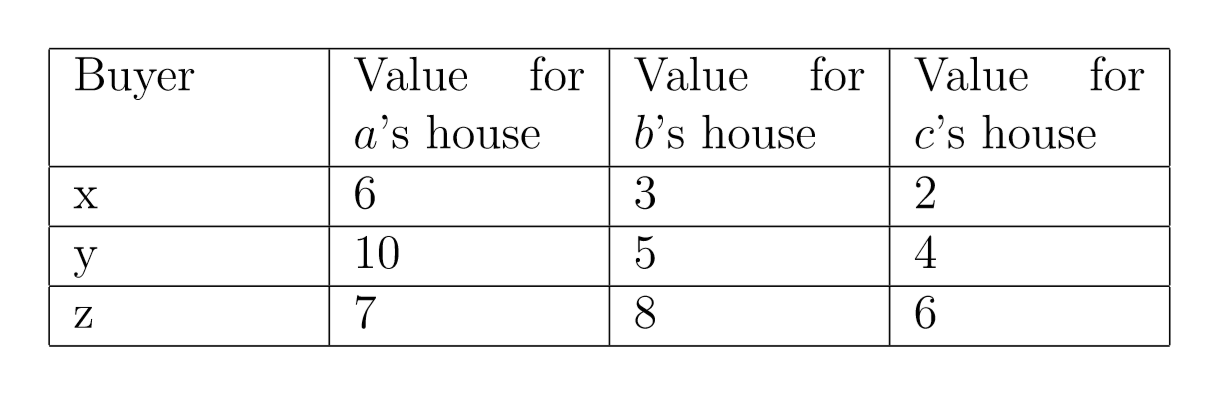
\includegraphics{Q6}
\caption{Buyer's valuations}
\end{figure}

We first calculate the payoff of each buyer for all the houses.

As we know that,

Payoff for a buyer = Buyer's valuation of the house - Price of the house

Let P(x,a) be the payoff of a buyer x for the seller a

Let P(x,b) be the payoff of a buyer x for the seller b and so on..

Therefore

P(x,a) = 2 , P(y,a) = 6 , P(z,a) = 3

P(x,b) = 2 , P(y,b) = 4,  P(z,b) = 7

P(x,c) = 2 , P(z,b) = 4,  P(z,c) = 6


The figure below shows a preferred-seller graph for the buyers and sellers where the buyers are connected to the sellers that give them the maximum payoff.

{\centering
 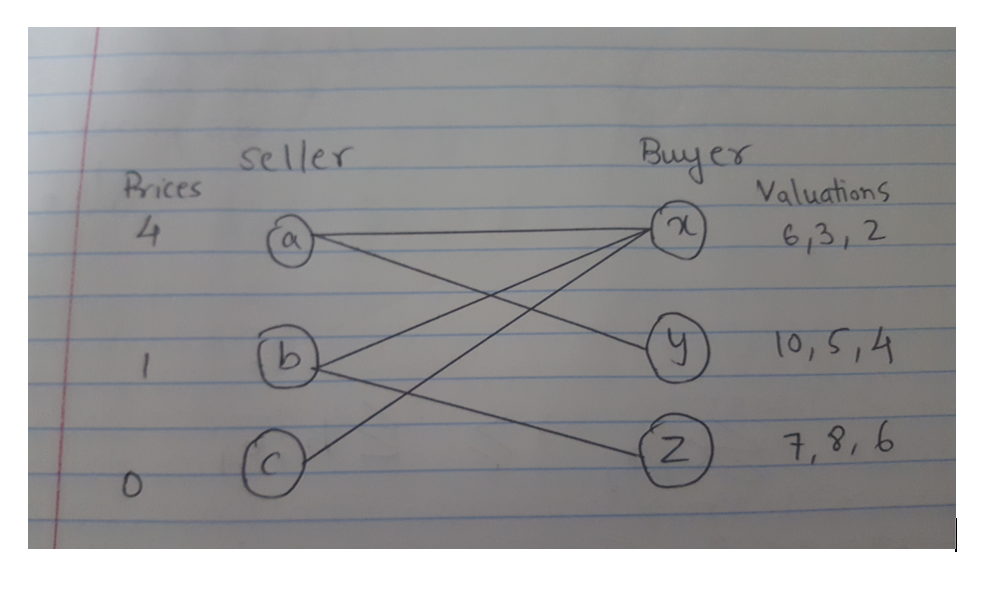
\includegraphics{Q6-1}\par
}


As we can see from the graph above that for buyer y, seller a is the preferred seller (since seller a gives this buyer the maximum payoff).

Also, for buyer z, seller b is the preferred seller (since seller b gives this buyer the maximum payoff).

Hence, buyer y must get the house from seller a and buyer z must get the house from seller b.

As we can see that there is no seller that gives a maximum payoff to the buyer x, since all the three sellers give an equal payoff of 2 to the buyer x. Hence, buyer x would get the house from seller c.

Also, since each house is now bought by a different buyer, the set of prices we have here are market-clearing prices. The market clearing value is [4,1,0]



\textbf{Question 7}.

In this question we have been given a set of 3 sellers a, b and c offering their houses for sale and a set of 3 buyers x, y and z having their own valuations for each of the houses. The figure below shows the valuations of each buyer for each of the houses:

\begin{figure}[htp]
\centering
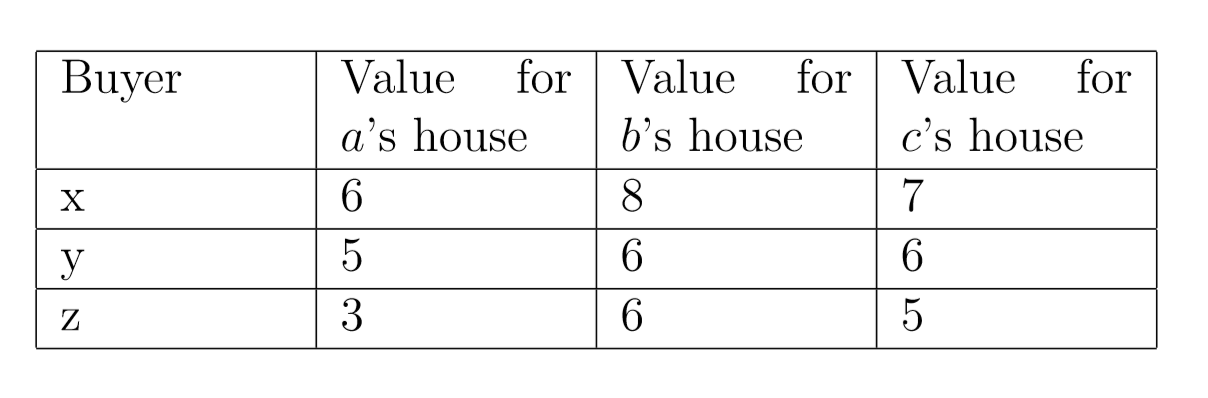
\includegraphics{Q7}
\caption{Buyer's valuations}
\end{figure}

Based on the buyer's valuations for each houses and their actual prices, we match each buyer on the right with its preferred seller or sellers on the left. A preferred seller is the one which gives the highest payoff to a buyer.


{\centering
 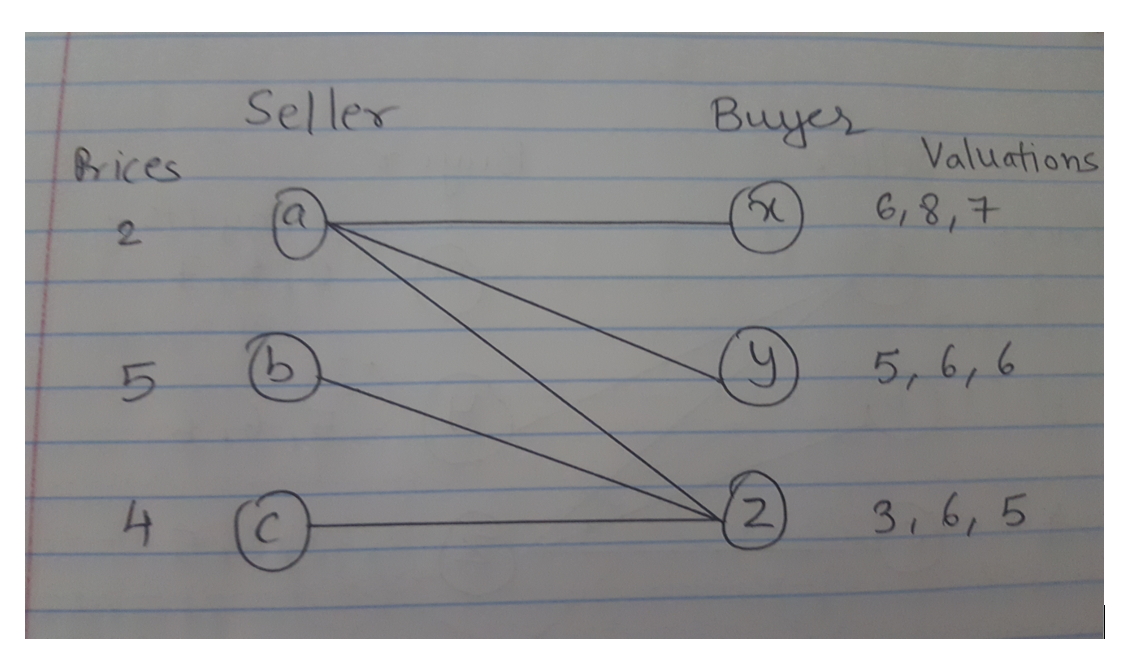
\includegraphics{Q7-1}\par
}
Based on the above graph, we see that since seller 'a' is the preferred seller for both x and y, we know that the above set of prices are not market clearing since we have a constricted set S= {x,y} of buyers that prefer the same seller, N(S)={a}.

Hence, to make these prices market clearing, we increase the price of a by 1. So, the new prices become, a=3, b=5 and c=4. Hence the next round of the bipartite auction procedure is shown as follows:

\begin{figure}[htp]
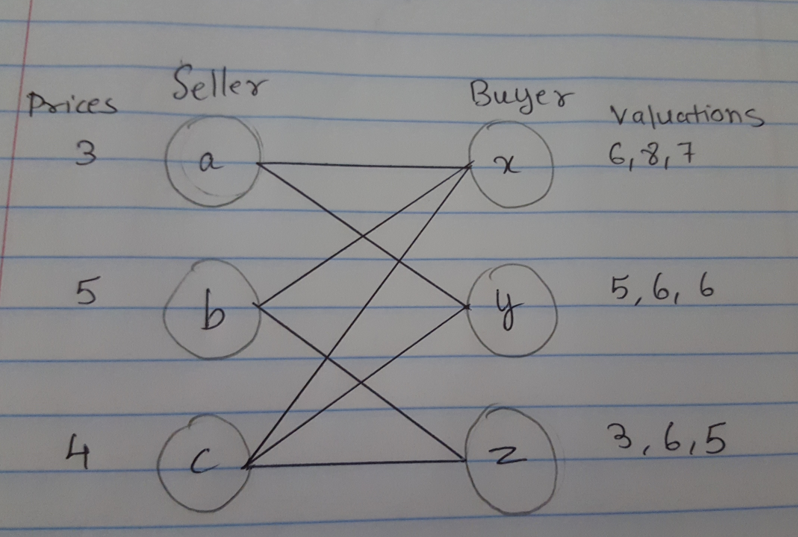
\includegraphics{q7_2}
\centering
\caption{Bipartite graph after increasing the price for seller a}
\end{figure}

From the above graph we can see that buyer x has a payoff of 3 for all the houses, hence x could go with any of the three houses.
Buyer y has a payoff of 2 with seller a and c. Hence, y could go with either seller a or c. Buyer z has a payoff of 1 for seller b and c. Hence, z could go with seller b or c.

Hence, there are three possible ways in which the buyers could be matched with the sellers:
 
 1)  [(x,c),(y,a),(z,b)] or
 
 2)  [(x,b),(y,a),(z,c)] or
 
 3)  [(x,a),(y,c),(z,b)]
 
 Hence, the market clearing price for the above set of buyers and sellers is [3,5,4]

\end{document}





